%%%%%%%%%%%%%%%%%%%%%%%%%%%%%%%%%%%%%%%%%
% LaTeX Template
%
% This template originates from:
% http://www.LaTeXTemplates.com
%
% License:
% CC BY-NC-SA 3.0 (http://creativecommons.org/licenses/by-nc-sa/3.0/)
% 
%%%%%%%%%%%%%%%%%%%%%%%%%%%%%%%%%%%%%%%%%

%----------------------------------------------------------------------------------------
%	PACKAGES AND OTHER DOCUMENT CONFIGURATIONS
%----------------------------------------------------------------------------------------

\documentclass{article}

%%%%%%%%%%%%%%%%%%%%%%%%%%%%%%%%%%%%%%%%%
% Lachaise Assignment
% Structure Specification File
% Version 1.0 (26/6/2018)
%
% This template originates from:
% http://www.LaTeXTemplates.com
%
% Authors:
% Marion Lachaise & François Févotte
% Vel (vel@LaTeXTemplates.com)
%
% License:
% CC BY-NC-SA 3.0 (http://creativecommons.org/licenses/by-nc-sa/3.0/)
% 
%%%%%%%%%%%%%%%%%%%%%%%%%%%%%%%%%%%%%%%%%

%----------------------------------------------------------------------------------------
%	PACKAGES AND OTHER DOCUMENT CONFIGURATIONS
%----------------------------------------------------------------------------------------

\usepackage{amsmath,amsfonts,stmaryrd,amssymb} % Math packages

\usepackage{enumerate} % Custom item numbers for enumerations

\usepackage[ruled]{algorithm2e} % Algorithms

\usepackage[framemethod=tikz]{mdframed} % Allows defining custom boxed/framed environments

\usepackage{listings} % File listings, with syntax highlighting
\lstset{
	basicstyle=\ttfamily, % Typeset listings in monospace font
}

%----------------------------------------------------------------------------------------
%	DOCUMENT MARGINS
%----------------------------------------------------------------------------------------

\usepackage{geometry} % Required for adjusting page dimensions and margins

\geometry{
	paper=a4paper, % Paper size, change to letterpaper for US letter size
	top=2.5cm, % Top margin
	bottom=3cm, % Bottom margin
	left=2.5cm, % Left margin
	right=2.5cm, % Right margin
	headheight=14pt, % Header height
	footskip=1.5cm, % Space from the bottom margin to the baseline of the footer
	headsep=1.2cm, % Space from the top margin to the baseline of the header
	%showframe, % Uncomment to show how the type block is set on the page
}

%----------------------------------------------------------------------------------------
%	FONTS
%----------------------------------------------------------------------------------------

\usepackage[utf8]{inputenc} % Required for inputting international characters
\usepackage[T1]{fontenc} % Output font encoding for international characters

\usepackage{XCharter} % Use the XCharter fonts

%----------------------------------------------------------------------------------------
%	COMMAND LINE ENVIRONMENT
%----------------------------------------------------------------------------------------

% Usage:
% \begin{commandline}
%	\begin{verbatim}
%		$ ls
%		
%		Applications	Desktop	...
%	\end{verbatim}
% \end{commandline}

\mdfdefinestyle{commandline}{
	leftmargin=10pt,
	rightmargin=10pt,
	innerleftmargin=15pt,
	middlelinecolor=black!50!white,
	middlelinewidth=2pt,
	frametitlerule=false,
	backgroundcolor=black!5!white,
	frametitle={Command Line},
	frametitlefont={\normalfont\sffamily\color{white}\hspace{-1em}},
	frametitlebackgroundcolor=black!50!white,
	nobreak,
}

% Define a custom environment for command-line snapshots
\newenvironment{commandline}{
	\medskip
	\begin{mdframed}[style=commandline]
}{
	\end{mdframed}
	\medskip
}

%----------------------------------------------------------------------------------------
%	FILE CONTENTS ENVIRONMENT
%----------------------------------------------------------------------------------------

% Usage:
% \begin{file}[optional filename, defaults to "File"]
%	File contents, for example, with a listings environment
% \end{file}

\mdfdefinestyle{file}{
	innertopmargin=1.6\baselineskip,
	innerbottommargin=0.8\baselineskip,
	topline=false, bottomline=false,
	leftline=false, rightline=false,
	leftmargin=2cm,
	rightmargin=2cm,
	singleextra={%
		\draw[fill=black!10!white](P)++(0,-1.2em)rectangle(P-|O);
		\node[anchor=north west]
		at(P-|O){\ttfamily\mdfilename};
		%
		\def\l{3em}
		\draw(O-|P)++(-\l,0)--++(\l,\l)--(P)--(P-|O)--(O)--cycle;
		\draw(O-|P)++(-\l,0)--++(0,\l)--++(\l,0);
	},
	nobreak,
}

% Define a custom environment for file contents
\newenvironment{file}[1][File]{ % Set the default filename to "File"
	\medskip
	\newcommand{\mdfilename}{#1}
	\begin{mdframed}[style=file]
}{
	\end{mdframed}
	\medskip
}

%----------------------------------------------------------------------------------------
%	NUMBERED QUESTIONS ENVIRONMENT
%----------------------------------------------------------------------------------------

% Usage:
% \begin{question}[optional title]
%	Question contents
% \end{question}

\mdfdefinestyle{question}{
	innertopmargin=1.2\baselineskip,
	innerbottommargin=0.8\baselineskip,
	roundcorner=5pt,
	nobreak,
	singleextra={%
		\draw(P-|O)node[xshift=1em,anchor=west,fill=white,draw,rounded corners=5pt]{%
		Question \theQuestion\questionTitle};
	},
}

\newcounter{Question} % Stores the current question number that gets iterated with each new question

% Define a custom environment for numbered questions
\newenvironment{question}[1][\unskip]{
	\bigskip
	\stepcounter{Question}
	\newcommand{\questionTitle}{~#1}
	\begin{mdframed}[style=question]
}{
	\end{mdframed}
	\medskip
}

%----------------------------------------------------------------------------------------
%	WARNING TEXT ENVIRONMENT
%----------------------------------------------------------------------------------------

% Usage:
% \begin{warn}[optional title, defaults to "Warning:"]
%	Contents
% \end{warn}

\mdfdefinestyle{warning}{
	topline=false, bottomline=false,
	leftline=false, rightline=false,
	nobreak,
	singleextra={%
		\draw(P-|O)++(-0.5em,0)node(tmp1){};
		\draw(P-|O)++(0.5em,0)node(tmp2){};
		\fill[black,rotate around={45:(P-|O)}](tmp1)rectangle(tmp2);
		\node at(P-|O){\color{white}\scriptsize\bf !};
		\draw[very thick](P-|O)++(0,-1em)--(O);%--(O-|P);
	}
}

% Define a custom environment for warning text
\newenvironment{warn}[1][Warning:]{ % Set the default warning to "Warning:"
	\medskip
	\begin{mdframed}[style=warning]
		\noindent{\textbf{#1}}
}{
	\end{mdframed}
}

%----------------------------------------------------------------------------------------
%	INFORMATION ENVIRONMENT
%----------------------------------------------------------------------------------------

% Usage:
% \begin{info}[optional title, defaults to "Info:"]
% 	contents
% 	\end{info}

\mdfdefinestyle{info}{%
	topline=false, bottomline=false,
	leftline=false, rightline=false,
	nobreak,
	singleextra={%
		\fill[black](P-|O)circle[radius=0.4em];
		\node at(P-|O){\color{white}\scriptsize\bf i};
		\draw[very thick](P-|O)++(0,-0.8em)--(O);%--(O-|P);
	}
}

% Define a custom environment for information
\newenvironment{info}[1][Info:]{ % Set the default title to "Info:"
	\medskip
	\begin{mdframed}[style=info]
		\noindent{\textbf{#1}}
}{
	\end{mdframed}
}
 % Include the file specifying the document structure and custom commands

\usepackage{graphicx}
%Path in Windows format:
\graphicspath{ {.Images/} }

\newtheorem{definition}{Definition}[section]
\newtheorem{theorem}{Theorem}[section]

\usepackage{listings}
\usepackage{color}

\definecolor{dkgreen}{rgb}{0,0.6,0}
\definecolor{gray}{rgb}{0.5,0.5,0.5}
\definecolor{mauve}{rgb}{0.58,0,0.82}

\lstset{frame=tb,
  language=Python,
  aboveskip=3mm,
  belowskip=3mm,
  showstringspaces=false,
  columns=flexible,
  basicstyle={\small\ttfamily},
  numbers=none,
  numberstyle=\tiny\color{gray},
  keywordstyle=\color{blue},
  commentstyle=\color{dkgreen},
  stringstyle=\color{mauve},
  breaklines=true,
  breakatwhitespace=true,
  tabsize=3
}

\usepackage[titletoc]{appendix}

%----------------------------------------------------------------------------------------
%	ASSIGNMENT INFORMATION
%----------------------------------------------------------------------------------------

\title{Wheel of Fortune - Theory} % Title of the assignment

\author{Tansel Arif\\ \texttt{tanselarif@live.co.uk}} % Author name and email address

\date{\today} % University, school and/or department name(s) and a date

%----------------------------------------------------------------------------------------

\begin{document}

\maketitle % Print the title

%----------------------------------------------------------------------------------------
%	INTRODUCTION
%----------------------------------------------------------------------------------------

\section*{Introduction} % Unnumbered section

\begin{flushleft}
It is sometimes the case that a random variable is dependent upon another random variable. For example, on some slot machines, the number of spins of the bonus wheel depends on the number of spin/bonus icons you achieve on the slots wheel itself. If you get 1 spin icon you get to spin the wheel once, if you get 2 spin icons, you get to spin the wheel twice and so on. If there is a certain probability of winning the bonus in the wheel each time you spin it and the wins from each spin are independent, then the more times you're allowed to spin it, the more chance of winning the bonus. But, the number of initial spin icons determines the number of times you're allowed to spin the wheel which in turn give you more chances to win the bonus. The question is, what is the probability of winning the bonus each time you play?\newline

Additionally, suppose the probability distribution of the slots is known but not that of the wheel. Given observations on the history of the games played and the results of those games, it is possible to make some guess on the probability distribution of the wheel that would most likely result in such data. We will approach this part of the problem by thinking in a Bayesian context.\newline

Below, I frame a similar problem with a wheel and coin flips to simplify the work a little.
\end{flushleft}

\section{The Problem} % Numbered section

\begin{flushleft}
You spin the wheel of fortune. The wheel gives $0$ with probability $\frac{1}{20}$, 1 with probability $\frac{1}{2}$, 2 with probability $\frac{1}{4}$, 3 with probability $\frac{3}{20}$ and 4 with probability $\frac{1}{20}$.\newline

Depending on the number you get from the wheel, you are allowed to flip a coin that many times and record the number of heads you get. The coin is biased towards heads with a probability of $\frac{7}{10}$ of getting a heads.\newline

What is the probability distribution of the number of heads if you play the game?
\end{flushleft}

\section{The Solution} % Numbered section

\begin{flushleft}
Let $W$ be a random variable (RV) representing the number obtained from spinning the wheel. Its distribution is shown in Figure \ref{fig:Wpf}. \newline

\begin{figure}
    \centering
    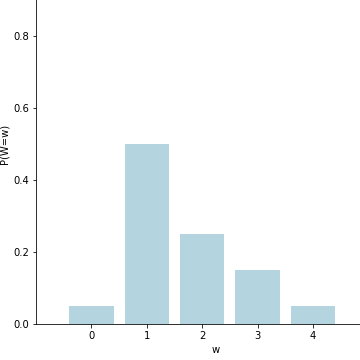
\includegraphics[scale=0.5]{Wpdf.png}
    \caption{This is the probability mass function for $W$.}
    \label{fig:Wpf}
\end{figure}

Let $X_i$ be independent and identically distributed (i.i.d) RVs representing the outcome of a flip of the coin. Then $X_i \sim Ber(p)$ where $p=0.7$ (i.e. each $X_i$ is a Bernoulli random variable with probability of success $p$).\newline

Define a RV, $Y$, as
$$Y = \sum_{i=1}^W X_i$$
where $W$ itself is random. We can approach this problem using probability generating functions (p.g.f):\newline

\begin{definition}{Probability Generating Function}{\label{label:pgf}}
If $X$ is a discrete RV taking values in the non-negative integers \{0,1,2,3,...\}, then the probability generating function of $X$ is defined as \cite{wikipediapgf}
$$G_X(s) = E(s^X) = \sum_{k=0}^{\infty} s^k P(X=k)$$
\end{definition}

Moreover,

\begin{theorem}[Uniqueness of p.g.f]{\label{thm:pgf}}
The distribution of a RV is uniquely determined by its p.g.f.
\end{theorem}

So let's find the p.g.f of $W$. From Definition \ref{label:pgf}:

\begin{equation} \label{eq1}
\begin{split}
G_W(s) & = E(s^W) \\
& = \sum_{k=0}^4 s^k P(W=k) \\
& = s^0 P(W=0) + s^1 P(W=1) + s^2 P(W=2) + s^3 P(W=3) + s^4 P(W=4) \\
& = \frac{1}{20} + \frac{1}{2}s + \frac{1}{4}s^2 + \frac{3}{20}s^3 + \frac{1}{20}s^4
\end{split}
\end{equation}

The p.g.f of $X \sim Ber(p)$ is

\begin{equation} \label{eqn:bernpgf}
\begin{split}
G_X(s) & = E(s^X) \\
& = \sum_{k=0}^1 s^k P(X=k) \\
& = s^0 P(X=0) + s^1 P(X=1)\\
& = 1-p + sp
\end{split}
\end{equation}

and the p.g.f of $Y = \sum_{i=1}^W X_i$ is 

\begin{equation} \label{eq1}
\begin{split}
G_Y(s) & = E(s^Y) \\
& = E(s^{\sum_{i=1}^W X_i}) \\
& = \sum_{w=0}^4 E(s^{\sum_{i=1}^W X_i} | W=w) P(W=w) \\
& = \sum_{w=0}^4 E(s^{\sum_{i=1}^w X_i}) P(W=w) \\
& = \sum_{w=0}^4 E(\Pi_{i=1}^w s^{X_i}) P(W=w) \\
& = \sum_{w=0}^4 \Pi_{i=1}^w E(s^{X_i}) P(W=w) \\
& = \sum_{w=0}^4 \Pi_{i=1}^w G_X(s) P(W=w) \\
& = \sum_{w=0}^4 G_X(s)^w P(W=w) \\
& = E(G_X(s)^W) \\
& = G_W(G_X(s))
\end{split}
\end{equation}

where the third line is the law of total probability, the fourth line is due to the RVs $X_i$ not depending on $W$ and the sixth line comes from the independence of the $X_i$s. Using equations 1 and 2 and collecting powers of $s$

\begin{equation} \label{eqn:gy}
\begin{split}
G_Y(s) & = \frac{1}{20} + \frac{1}{2}(1-p) + \frac{1}{4}(1-p)^2 + \frac{3}{20}(1-p)^3 + \frac{1}{20}(1-p)^4 \\
& + sp(\frac{1}{2} + \frac{1}{2}(1-p) + \frac{9}{20}(1-p)^2 + \frac{1}{5}(1-p)^3) \\
& + s^2 p^2(\frac{1}{4} + \frac{9}{20}(1-p) + \frac{3}{10}(1-p)^2) \\
& + s^3 p^3(\frac{3}{20} + \frac{1}{5}(1-p)) \\
& + s^4 p^4 \frac{1}{20}
\end{split}
\end{equation}

Keeping Definition \ref{label:pgf} in mind, the coefficient of $s^i$ in Equation \ref{eqn:gy} is $P(Y=i)$. The probability distribution of $Y$ is then

\begin{equation} \label{eqn:finalY}
\begin{split}
P(Y = 0) & = \frac{1}{20} + \frac{1}{2}(1-p) + \frac{1}{4}(1-p)^2 + \frac{3}{20}(1-p)^3 + \frac{1}{20}(1-p)^4 \\
P(Y = 1) & = p(\frac{1}{2} + \frac{1}{2}(1-p) + \frac{9}{20}(1-p)^2 + \frac{1}{5}(1-p)^3) \\
P(Y = 2) & = p^2(\frac{1}{4} + \frac{9}{20}(1-p) + \frac{3}{10}(1-p)^2) \\
P(Y = 3) & = p^3(\frac{3}{20} + \frac{1}{5}(1-p)) \\
P(Y = 4) & = p^4 \frac{1}{20}
\end{split}
\end{equation}

Notice that if the probability of heads in the coin flip is 1 (p = 1), we recover the probability distribution of $W$, i.e. $W$ completely determines the number of heads.\newline

Conversely, if the probability of heads in the coin flip is 0 (p = 0), the coin will always land tails regardless of the outcome of a trial from $W$. Then $P(Y=0) = 1$, i.e. no matter what happens, there will be no heads from the game.\newline

So, to answer the original question, we plug $p=0.7$ into Equation \ref{eqn:finalY} to obtain the following distribution for the number of heads:

\begin{equation} \label{dist:finalY}
\begin{split}
P(Y = 0) & = 0.226955\\
P(Y = 1) & = 0.48713\\
P(Y = 2) & = 0.20188\\
P(Y = 3) & = 0.07203\\
P(Y = 4) & = 0.012005
\end{split}
\end{equation}

\end{flushleft}
\section{Finding the probability $p$ from observations} % Numbered section

\begin{flushleft}
Suppose that we are not told the value of $p$. Given an observation of $W$, $Y$ has a more well-known distribution

$$Y = \sum_{i=0}^w X_i$$

In particular, $Y$ is just the sum of independent Bernoulli ($Ber(p)$) RVs which has a binomial distribution

$$Y \sim B(w,p)$$

(See section \ref{sec:bin} for proof using p.g.f definitions above). In mathematical notation, the above means

$$Y|W=w \sim B(w,p)$$

Let $p \sim Beta(\alpha, \beta)$ for some $\alpha$ $\beta$. I have chosen this distribution for $p$ as this is conjugate to the Binomial Distribution (see section \ref{sec:conj}) which makes calculations easier.\newline

The posterior distribution for $p$ can then be written as

\begin{equation} \label{eqp}
\begin{split}
P(p|Y,W) & = \frac{P(p,Y,W)}{P(Y,W)} \\
& = \frac{P(Y|W,p) P(W) P(p)}{\sum_{w=0}^4 P(Y|W=w) P(W=w)} \\
& = Beta(p,\alpha + \sum_{i=1}^n y_i, \beta + \sum_{i=1}^n w_i - \sum_{i=1}^n y_i)
\end{split}
\end{equation}

where in the last line we used the conjugacy property (see section \ref{sec:conj}). If we were just interested in finding the most likely value for $p$, we wouldn't have needed to restrict ourselves to conjugate priors since the calculation of the denominator in the second line of Equation \ref{eqp} would not be required; the main advantage of using conjugate priors in non-Monte Carlo scenarios. This would allow a larger variety of prior distributions for $p$.

Let us find the most likely distribution for $p$. In order to find $p$ which maximises $P(p|Y,W)$, we need only concern ourselves with the terms involving $p$. Using the definition of the $Beta$ distribution, we can write Equation \ref{eqp} as

\begin{equation} \label{eqmle}
\begin{split}
P(p|Y,W) & = K p^{\alpha'-1}(1-p)^{\beta'-1}
\end{split}
\end{equation}

where $K$ is a constant and

$$\alpha' = \alpha + \sum_{i=1}^N y_i,\; \beta' = \beta + \sum_{i=1}^N w_i - \sum_{i=1}^N y_i$$

Taking the derivative of Equation \ref{eqmle} with respect to $p$

\begin{equation} \label{eqmle2}
\begin{split}
\frac{\partial P(p|Y,W)}{\partial p} & = \left[  (\alpha' - 1)p^{\alpha'-2} (1-p)^{\beta'-1} - p^{\alpha'-1}(\beta'-1)(1-p)^{\beta'-2}  \right]
\end{split}
\end{equation}

Replacing $\alpha'$ and $\beta'$, and setting this equal to zero we obtain

\begin{equation} \label{eqmle3}
\begin{split}
p &= \frac{1-\alpha'}{2-\alpha'-\beta'} \\
&= \frac{1-(\alpha + \sum_{i=1}^N y_i)}{2-(\alpha + \sum_{i=1}^N y_i)-(\beta - \sum_{i=1}^N w_i - \sum_{i=1}^N y_i)} \\
&= \frac{1-(\alpha + \sum_{i=1}^N y_i)}{2-\alpha-\beta-\sum_{i=1}^N w_i}
\end{split}
\end{equation}

Equation \ref{eqmle3} gives us a way of calculating the value of $p$ that is most likely given observations of $W$ and $Y$. Going further, the above assumes knowledge of the outcomes from $W$. If we don't have this information, the approximation $E[W] \approx \frac{1}{N}\sum_{i=1}^N w_i$ will help with an approximation. In this case we may utilise the expected value of $W$ to be used in Equation \ref{eqmle3} as follows

\begin{equation} \label{eqmle4}
\begin{split}
p &= \frac{1-(\alpha + \sum_{i=1}^N y_i)}{2-\alpha-\beta-N E[W]} \\
&\approx \frac{1-(\alpha + \sum_{i=1}^N y_i)}{2-\alpha-\beta-N \frac{\sum_{i=1}^N w_i}{N}}
\end{split}
\end{equation}

Let's see what happens when we set $p=2$ in the theory section above and provide `hypothetically ideal' observations to be used in Equation \ref{eqmle4}. The probability distribution of $Y$ then becomes

\begin{equation} \label{eqYpdf}
\begin{split}
P(Y=0) &= 0.70728 \\
P(Y=1) &= 0.25808 \\
P(Y=2) &= 0.03208 \\
P(Y=3) &= 0.00248 \\
P(Y=4) &= 0.00008
\end{split}
\end{equation}

According to \ref{eqYpdf}, out of $N=100000$ trials, we expect to have: $70728$ trials resulting in $0$ heads, $25808$ trials resulting in $1$ head, $3208$ trials resulting in $2$ heads, $248$ trials resulting in $3$ heads and $8$ trials resulting in $4$ heads for a total of $33000$ heads in $100000$ trials/games. Additionally, 

$$E[W] = 0*\frac{1}{20} + 1*\frac{1}{2} + 2*\frac{1}{4} + 3*\frac{3}{20} + 4*\frac{1}{20}=1.65$$

\begin{figure}
    \centering
    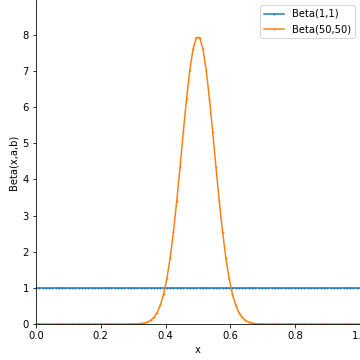
\includegraphics[scale=0.5]{Beta.png}
    \caption{This is the probability distribution of $Beta(1,1)$ and $Beta(50,50)$.}
    \label{fig:Beta}
\end{figure}

For the prior distribution for $p$, we may specify the parameters $\alpha=1$ and $\beta=1$ resulting in a $Beta$ distribution that is uniform without assuming any information about the unbias/bias nature of the coin. The prior distribution for $p$ is shown in blue in Figure \ref{fig:Beta}. Using these parameters, our estimation for the value of $p$ that was used to generate these observations is

$$p = \frac{1-(1+33000)}{-100000 \times 1.65} = 0.2$$

Note that here we have only used the knowledge of the outcomes along with the p.d.f of $W$ to determine $p$. We did not need to know the distribution of $Y$. In general, the p.d.f of $W$ may be unknown requiring the data from the outcomes of $W$, or there may be strong prior evidence that the coin is unbiased (we could set $\alpha = 50,\beta = 50$ for example to assume a strong prior around $p=0.5$ (see Figure \ref{fig:Beta})). Additionally, a posterior probability distribution for $p$ may be required, in which case we have $p \sim Beta(1+33000,1+1.65*100000-33000)$ shown in Figure \ref{fig:Beta2}.

\begin{figure}
    \centering
    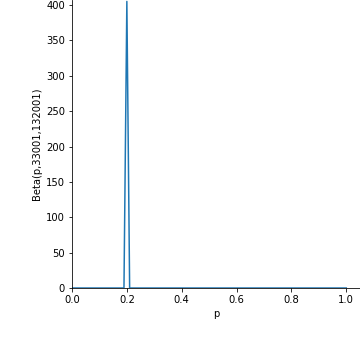
\includegraphics[scale=0.5]{Beta2.png}
    \caption{This is the posterior probability distribution for $p$.}
    \label{fig:Beta2}
\end{figure}

\end{flushleft}
\section{Simulations} % Numbered section
\begin{flushleft}
We can perform simulations of this process by first selecting a value, $w$, from the distribution for $W$ then selecting $w$ values from a Bernoulli distribution with specified probability of success $p$.\newline

Below shows Python code used for performing the simulation:

\begin{lstlisting}
# Import modules
from scipy import stats
import math
import numpy

# Set the seed
np.random.seed(101)

# Build W by concatenation of lists
w = []
w.append(0)
w.extend([1]*10+[2]*5+[3]*3+[4]*1)

# Set the probability of heads from a coin flip
p = 0.2

# Set the number of games
n = 10000

# Initialise the total number of heads obtained
y_outcome = 0

# Get n samples from w
w_outcome = np.random.choice(w,size=n)

# For each w, flip the coin that many times
y_outcome = [np.sum(stats.bernoulli.rvs(p,size=this_w)) for this_w in w_outcome]

y_sum = sum(y_outcome)
w_sum = sum(w_outcome)

print('Total number of heads = {}'.format(y_sum))
print('Total number of coin flips = {}'.format(w_sum))

>>> Total number of heads = 3202
>>> Total number of coin flips = 16536
\end{lstlisting}

Next we plot a representation of the posterior distribution for $p$ using the theory in the previous section.

\begin{lstlisting}
# Get figure object
fig = plt.figure(figsize=(5, 5))

# Get aces object
axes = fig.add_axes([0.2,0.2,0.8,0.8])

# Create a numpy array of 100 points equally spaced
x = np.linspace(0,1,100)

# Create a numpy array of the posterior distribution using actual observed values of W
y = np.array([stats.beta.pdf(i,1+y_sum,1-y_sum+w_sum) for i in x])

# Create a numpy array of the posterior distribution by estimating sum(W) with it's expected value
z = np.array([stats.beta.pdf(i,1+y_sum,1-y_sum+n*1.65) for i in x])

# Plot onto the axes
axes.plot(x, y, '-o',ms=0,label='Using data from W')
axes.plot(x, z, '-o',ms=0,label='Approximating sum(w_i) with n*E[W]')

# Set the axis labels
axes.set_xlabel('p')
axes.set_ylabel('Beta(p,a,b)')

# Show legend
axes.legend()

# Set axis limits
axes.set_xlim(0,1.05)
axes.set_ylim(0,max(y.max(),z.max())+10)

# Remove some borders
axes.spines['right'].set_visible(False)
axes.spines['top'].set_visible(False)
\end{lstlisting}

This produces the plots in Figure \ref{fig:BetaSim}. It can be seen that the posterior distribution correctly estimates the probability associated with getting a heads from the coin flip $p$ as $0.2$.

\begin{figure}
    \centering
    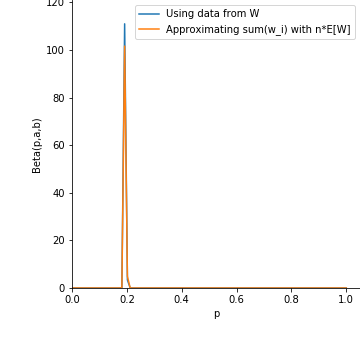
\includegraphics[scale=0.5]{BetaSimulation.png}
    \caption{A simulation is run by performing $n=10000$ trials of the process of spinning a wheel and flipping a coin a number of times specified by the value obtained from the wheel and summing the number of heads obtained throughout the simulation. The probability of heads is chosen as $p=0.2$. The theory resulting in Equation \ref{eqp} is used to generate both probability distributions in the plot. The blue line uses the data from the actual trials from $W$ whereas the orange line uses an estimated value for $W$ for cases where we only know the outcome $Y$.}
    \label{fig:BetaSim}
\end{figure}

\end{flushleft}

\newpage

\appendix

\section{The sum of $n$ Bernoulli random variables is a Binomial random variable}\label{sec:bin}

\begin{flushleft}

By Equation \ref{eqn:bernpgf}, the p.g.f of a Bernoulli RV $X$ is

$$G_X(s) = 1-p+sp$$

Similarly, using Definition \ref{label:pgf}, the p.g.f of a Binomial RV $Z$ such that $Z \sim B(n,p)$ and $P(Z=z;n,p) = {n \choose z} p^z (1-p)^{n-z}$ is

\begin{equation}
\begin{split}
G_Z(s) &= E[s^Z] \\
&= \sum_{z=0}^n s^z P(Z=z) \\
&= \sum_{z=0}^n s^z {n \choose z} p^z (1-p)^{n-z} \\
&= \sum_{z=0}^n {n \choose z} (sp)^z (1-p)^{n-z} \\
&= (sp +1 - p)^n
\end{split}
\end{equation}

where the last equality is from the identity $(a + b)^n = \sum_{i=0}^n {n \choose i}a^i b^{n-i}$. Let $Y = \sum_{i=0}^n X_i$, i.e. the RV $Y$ is the sum of the $n$ RVs $X_i$. Then the $p.g.f$ of $Y$ is

\begin{equation}
\begin{split}
G_Y(s) &= E[s^Y] \\
&= \sum_{y=0}^n s^y P(Y=y) \\
&= E[s^{\sum_{i=0}^n X_i}] \\
&= E[\Pi_{i=0}^n s^{X_i}] \\
&= \Pi_{i=0}^n E[s^{X_i}] \;\; \text{(since} \; X_i \; \text{are independent)}\\
&= (G_X(s))^n \;\; \text{(by the p.g.f of a Bernoulli RV}\\
&= (sp +1 - p)^n
\end{split}
\end{equation}

This p.g.f is the same as that of the Binomial RV above and by Theorem \ref{thm:pgf}, $Y \sim B(n,p)$.

\end{flushleft}

\section{Conjugacy property of $Y \sim B(n,p)$ and $p \sim Beta(\alpha, \beta)$}\label{sec:conj}

\begin{flushleft}

Let $W$ be a RV with a defined distribution with parameters specified. Let $Y \sim B(n,p)$ and prior $p \sim Beta(\alpha,\beta)$. Then

\begin{equation} \label{eqpapp}
\begin{split}
P(p|Y,W) & = \frac{P(p,Y,W)}{P(Y,W)} \\
& = \frac{P(Y|W,p) P(W) P(p)}{\sum_{w=0}^4 P(Y|W=w) P(W=w)} \\
& = \frac{P(Y_1 = y_1,Y_2 = y_2,...,Y_n = y_n|W,p) P(W) P(p)}{\sum_{w=0}^4 P(Y|W=w) P(W=w)} \\
& = \frac{P(Y_1 = y_1|W,p)...P(Y_n = y_n|W,p) P(W) P(p)}{\sum_{w=0}^4 P(Y|W=w) P(W=w)} \;\; \text{since the } Y_i \; \text{are independent}\\
& = \frac{P(Y_1 = y_1|W_1=w_1,p)...P(Y_n = y_n|W_n=w_n,p) P(W) P(p)}{\sum_{w=0}^4 P(Y|W=w) P(W=w)} \;\; \text{since } Y_i \; \text{depends only on } W_i\\
& = \frac{B(y_1;w_1,p)...B(y_n;w_n,p) P(W) Beta(p,\alpha,\beta)}{\sum_{w=0}^4 P(Y|W=w) P(W=w)}\\
& = \frac{{w_1 \choose y_1} p^{y_1} (1-p)^{w_1-y_1}...{w_n \choose y_n} p^{y_n} (1-p)^{w_n-y_n} P(W) \frac{\Gamma(\alpha+\beta)}{\Gamma(\alpha)\Gamma(\beta)}p^{\alpha-1}(1-p)^{\beta-1}}{\sum_{w=0}^4 P(Y|W=w) P(W=w)} \\
&= \frac{\frac{\Gamma(\alpha+\beta)}{\Gamma(\alpha)\Gamma(\beta)} P(W) \Pi_{i=0}^n \left[ {w_i \choose y_i} \right]}{\sum_{w=0}^4 P(Y|W=w) P(W=w)} p^{\sum_{i=0}^n y_i + \alpha - 1} (1-p)^{\sum_{i=0}^n (w_i - y_i) + \beta - 1}\\
&= K p^{\sum_{i=0}^n y_i + \alpha - 1} (1-p)^{\sum_{i=0}^n (w_i - y_i) + \beta - 1}
\end{split}
\end{equation}

The $K$ is a constant and not dependent upon $p$. Here, we note that the posterior distribution $P(p|Y,W)$ is itself a probability distribution and must sum/integrate to $1$. Since Equation \ref{eqpapp} has the form of a $Beta(p,\alpha + \sum_{i=1}^n y_i, \beta + \sum_{i=1}^n w_i - \sum_{i=1}^n y_i)$ distribution and must integrate to $1$, we have that $p|Y,W \sim Beta(\alpha + \sum_{i=1}^n y_i, \beta + \sum_{i=1}^n w_i - \sum_{i=1}^n y_i)$ and $K$ is a proportionality parameter which serves to scale the expression so that it has unit area. Here we have seen how a prior distribution for $p$ has been updated with data from the distribution for $Y$ resulting in a posterior distribution which remains within the same family as the prior distribution. The $Binomial$ and $Beta$ distributions thus have a property called Conjugacy.

\end{flushleft}

\newpage
\bibliographystyle{plain}
\bibliography{bibliography.bib}

%----------------------------------------------------------------------------------------
\end{document}
